\section{LA-CDIP Dataset Construction}
\label{sec:method_dataset}

\blue{The construction of this dataset is motivated by the absence of a specialized \gls{ZSL}-\gls{DIC} dataset, and the fact that \gls{RVL-CDIP} is unsuitable for the proposed \gls{VDM} method~\cite{khalifa_contrastive_2023} (see \refCap{sec:zsl-related}). To support \gls{VDM} in achieving \gls{ZSL}-\gls{DIC}, this dataset must provide two main characteristics: the dataset must provide great class diversity, so that models trained on this dataset can generalize across unseen classes. And the dataset must have consistent intra-class and inter-class consistency, so that the classes are atomic (with no possible subdivision).}

\blue{Therefore, the proposed dataset, \gls{LA-CDIP}, comes as reorganization of the \gls{RVL-CDIP} dataset, focusing on increased granularization, in the sense that no two document layouts are seen on the same class.} Visual cues such as a company logo, the layout of a table, the position of certain text, etc., all contribute to differentiating between distinct document patterns, and different patterns imply different classes. While the \gls{RVL-CDIP} dataset was used as source content, it was re-labeled to align with the problem of differentiating documents, with a particular focus on their visual structure (layout). \refFig{img:dataset} illustrates the impacts of the new labels. All eight documents in the figure used to belong to the same class, but now belong to two different classes under the new organization.

\begin{figure}[htbp]
  \centering
\includegraphics[width=.455\textwidth]{images/class_comparison1.png} \hspace{.04\textwidth}
    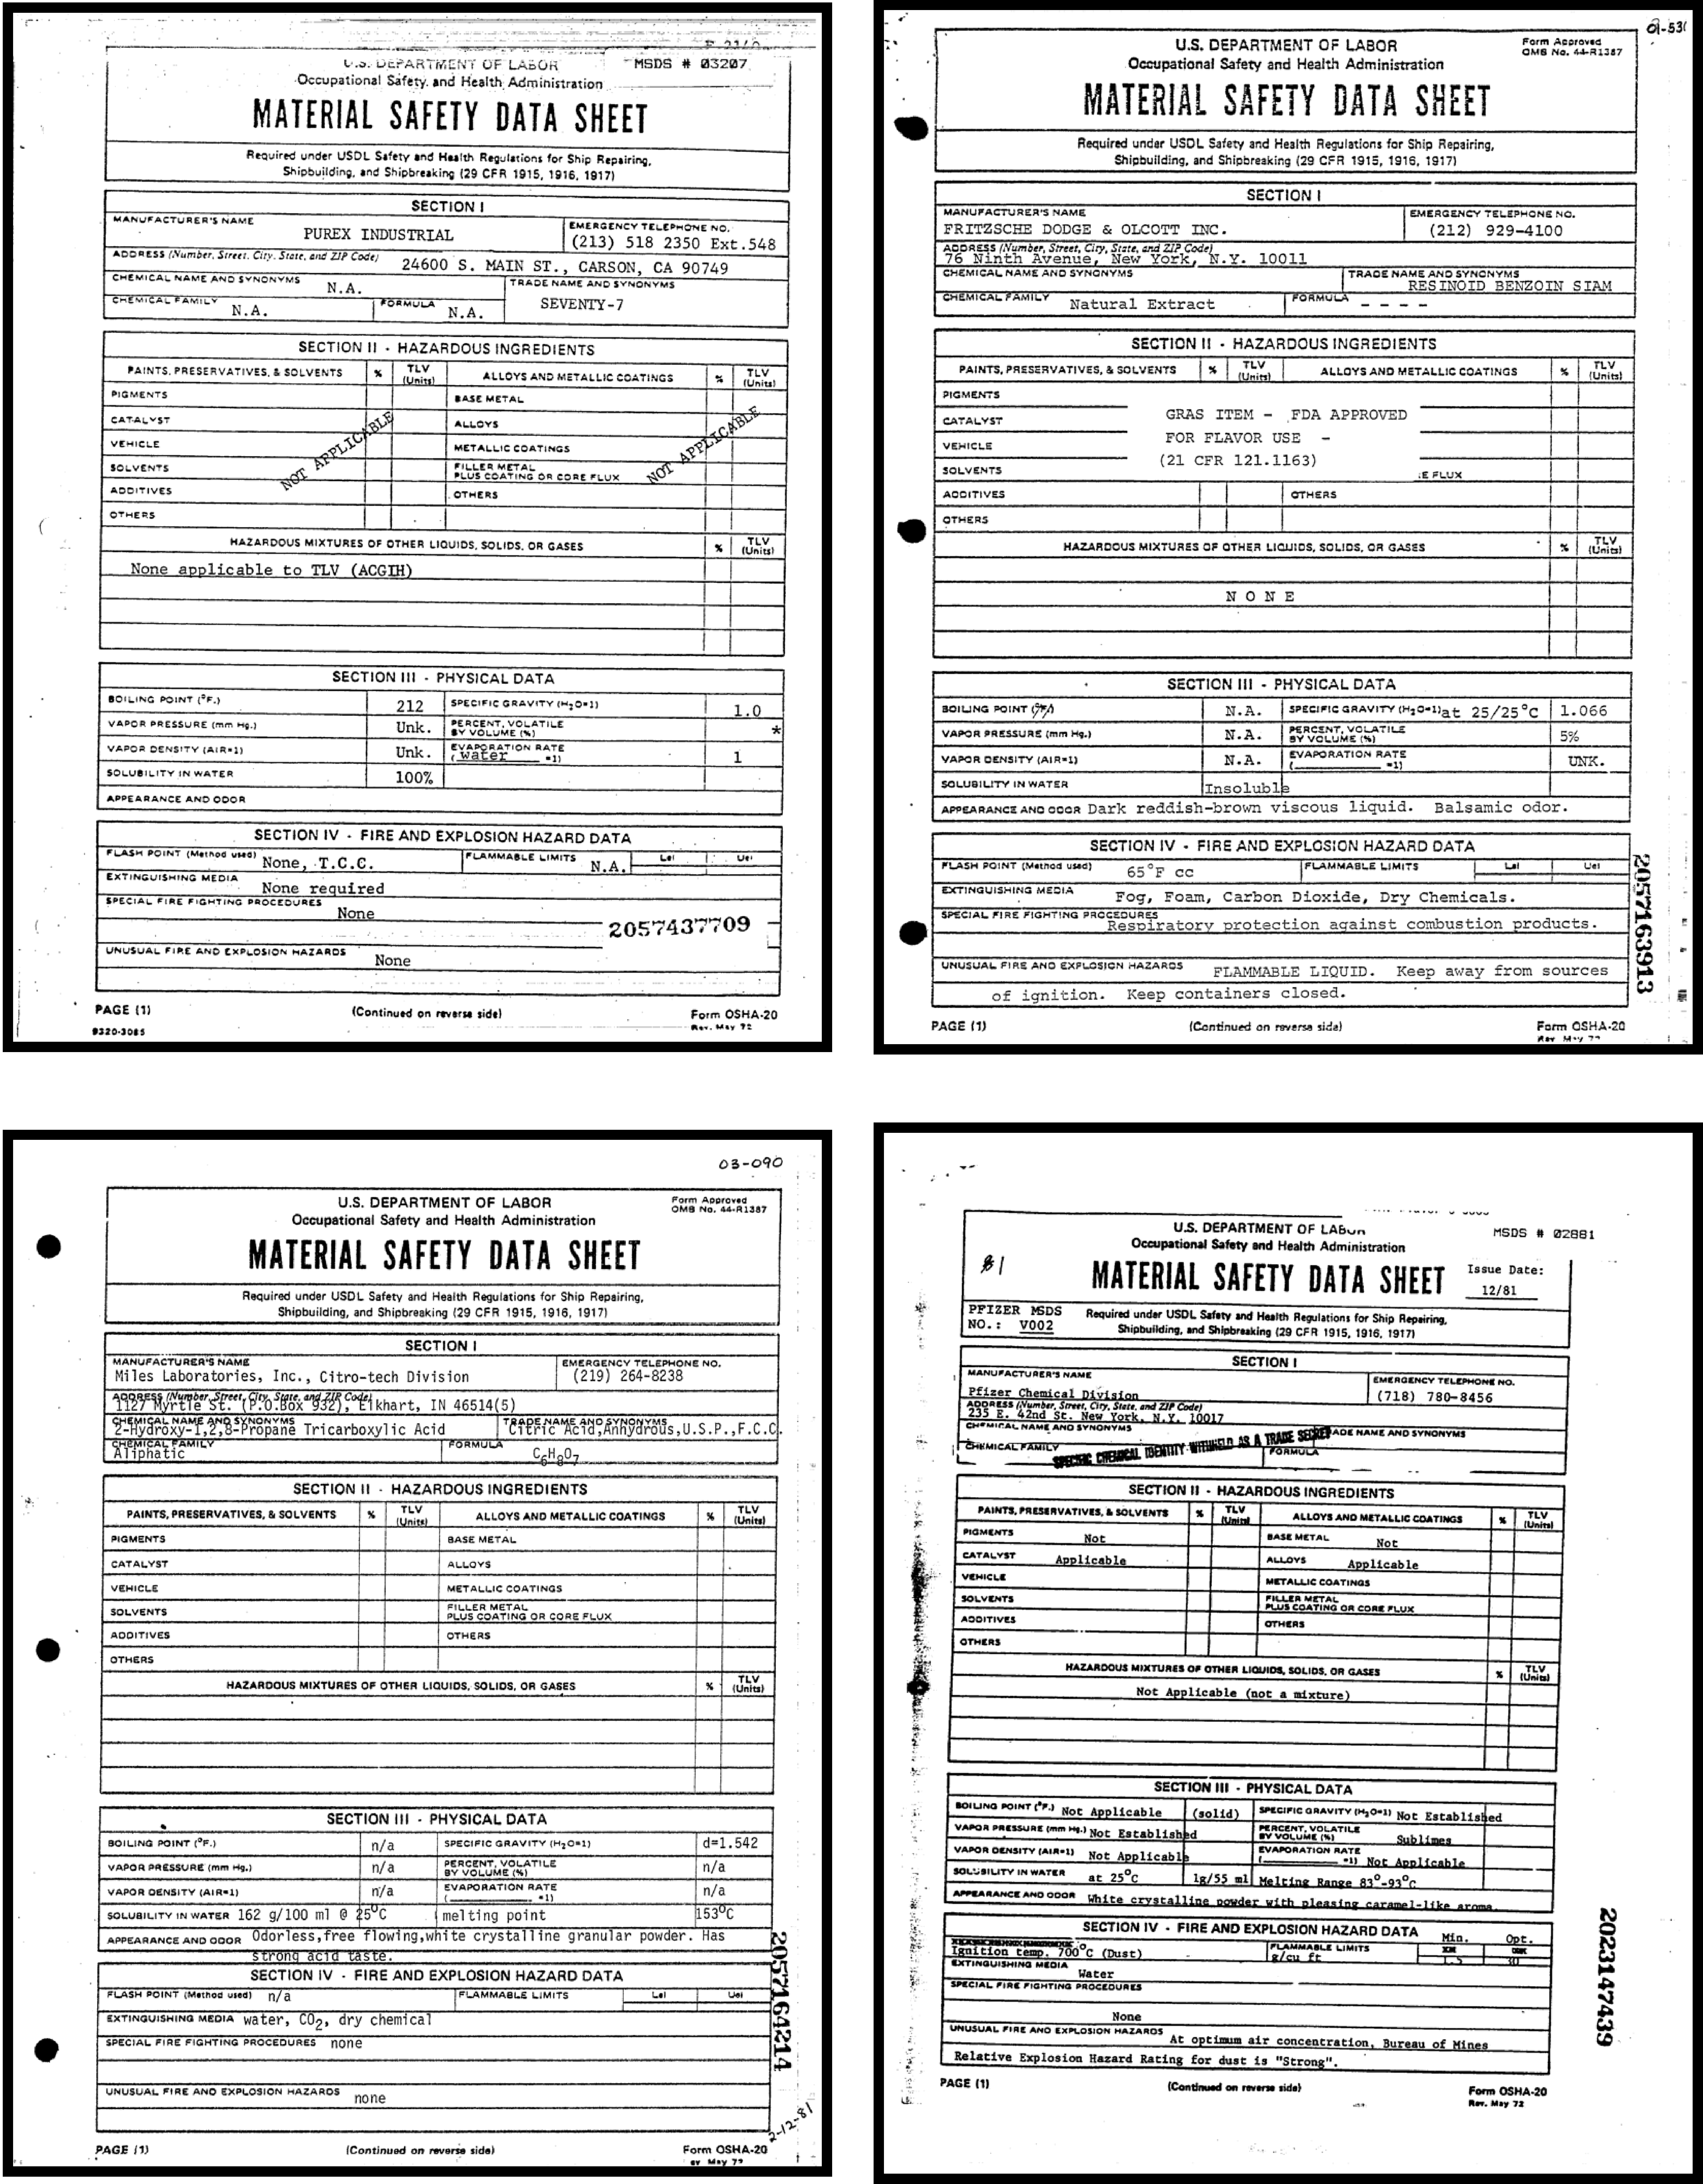
\includegraphics[width=.455\textwidth]{images/class_comparison2.png}

\caption{Examples of two distinct classes under the proposed \gls{LA-CDIP} dataset. Those classes originally belonged to the same class under RVL-CDIP organization.\label{img:dataset}}
\end{figure}   

%\red{The construction of the database followed a light active learning framework (see \refCap{sec:active_learning}), 
The dataset labeling following two stages: preliminary clustering, followed by a manual reorganization. The clustering is innitially made with a private metric learning model, trained with a private document dataset, with both the model and the dataset following the same methodology as this \blue{dissertation}. \blue{Following, the model is used to generate feature vectors across the entirety of the \gls{RVL-CDIP}. These feature vectors are then used to create clusters of documents, which are effectively predicted classes.} The Hierarchical Agglomerative Clustering algorithm, with Ward's\cite{ward_jr_hierarchical_1963} strategy is used (see \refCap{sec:clustering}). This clustering served the purpose of accelerating the manual labeling process.

\blue{The manual labeling process has two main tasks: first, verify the integrity of the clusters. As the clusters were made with a \gls{DL} model, they are prone to errors. Therefore, it is possible that one cluster holds many different document patters, which must be corrected by a human annotator, assuring intra-class consistency. Second, verify if this cluster is unique. The model may have created two distinct clusters with the same layout, therefore, a step to merge clusters is necessary, assuring inter-class consistency.}

\blue{This training pipeline is bound to a loop: given stop condition (which can be a time frame, or a goal in number of labeled documents), the annotated documents are comprised into a dataset, with more elements than the previous iteration, and are used to train a new model, using the same \gls{VDM} framework. This new, enhanced model is then used to create new clusters, which should have a greater intra-cluster and inter-cluster consistency, therefore, reducing the human annotation time necessary per document. To further optimize the labeling process, each cluster is ranked based on average pairwise distance between every element in the cluster, and the clusters with lowest average distances are provided first to the human annotators. This is meant to optimize the amount of work to achieve intra-class consistency.}

\begin{figure}[htbp]
\centering
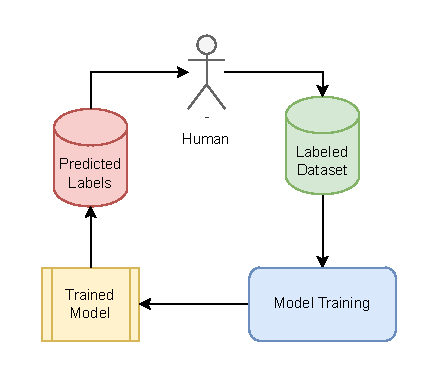
\includegraphics[width=.75\textwidth]{images/active_learning.drawio.pdf}
\caption{The proposed data labeling loop. Each loop, the labeled dataset is increased, which is used to train a better model, which results in more consistent predicted labels, reducing the time the human annotator spends per document.}
\label{fig:not_active_learning}
\end{figure}  

Note that the proposed data labeling loop is similar to active learning~\cite{settles_active_2009}, with a few key differences. While the \gls{LA-CDIP} dataset is created to support \gls{VDM}, it is still a contribution by itself. Therefore, the purpose of this labeling loop is to create a large and complete dataset, which differs from active learning philosophy, which is to achieve greater accuracy with fewer labeled instances~\cite{settles_active_2009}. The sampling strategy frequently used in active learning involves focusing the human efforts in samples that the model did not provide confidence in its classification, so that they provide the most value. This is opposite to what is proposed in this work, which is to give priority to clusters that have the most confidence, optimizing the time spent per annotation.

\section{LA-CDIP Dataset}
\label{sec:dataset}

\red{The proposed dataset is composed of 4993 documents, divided into 144 different classes. Each class has at least two documents, the biggest class has 497 documents, and the median size of the classes is 13, exposing an extra challenge in dealing with an unbalanced dataset. \refFig{fig:histplot} shows the class distribution.}

\begin{figure}[htbp]
\centering
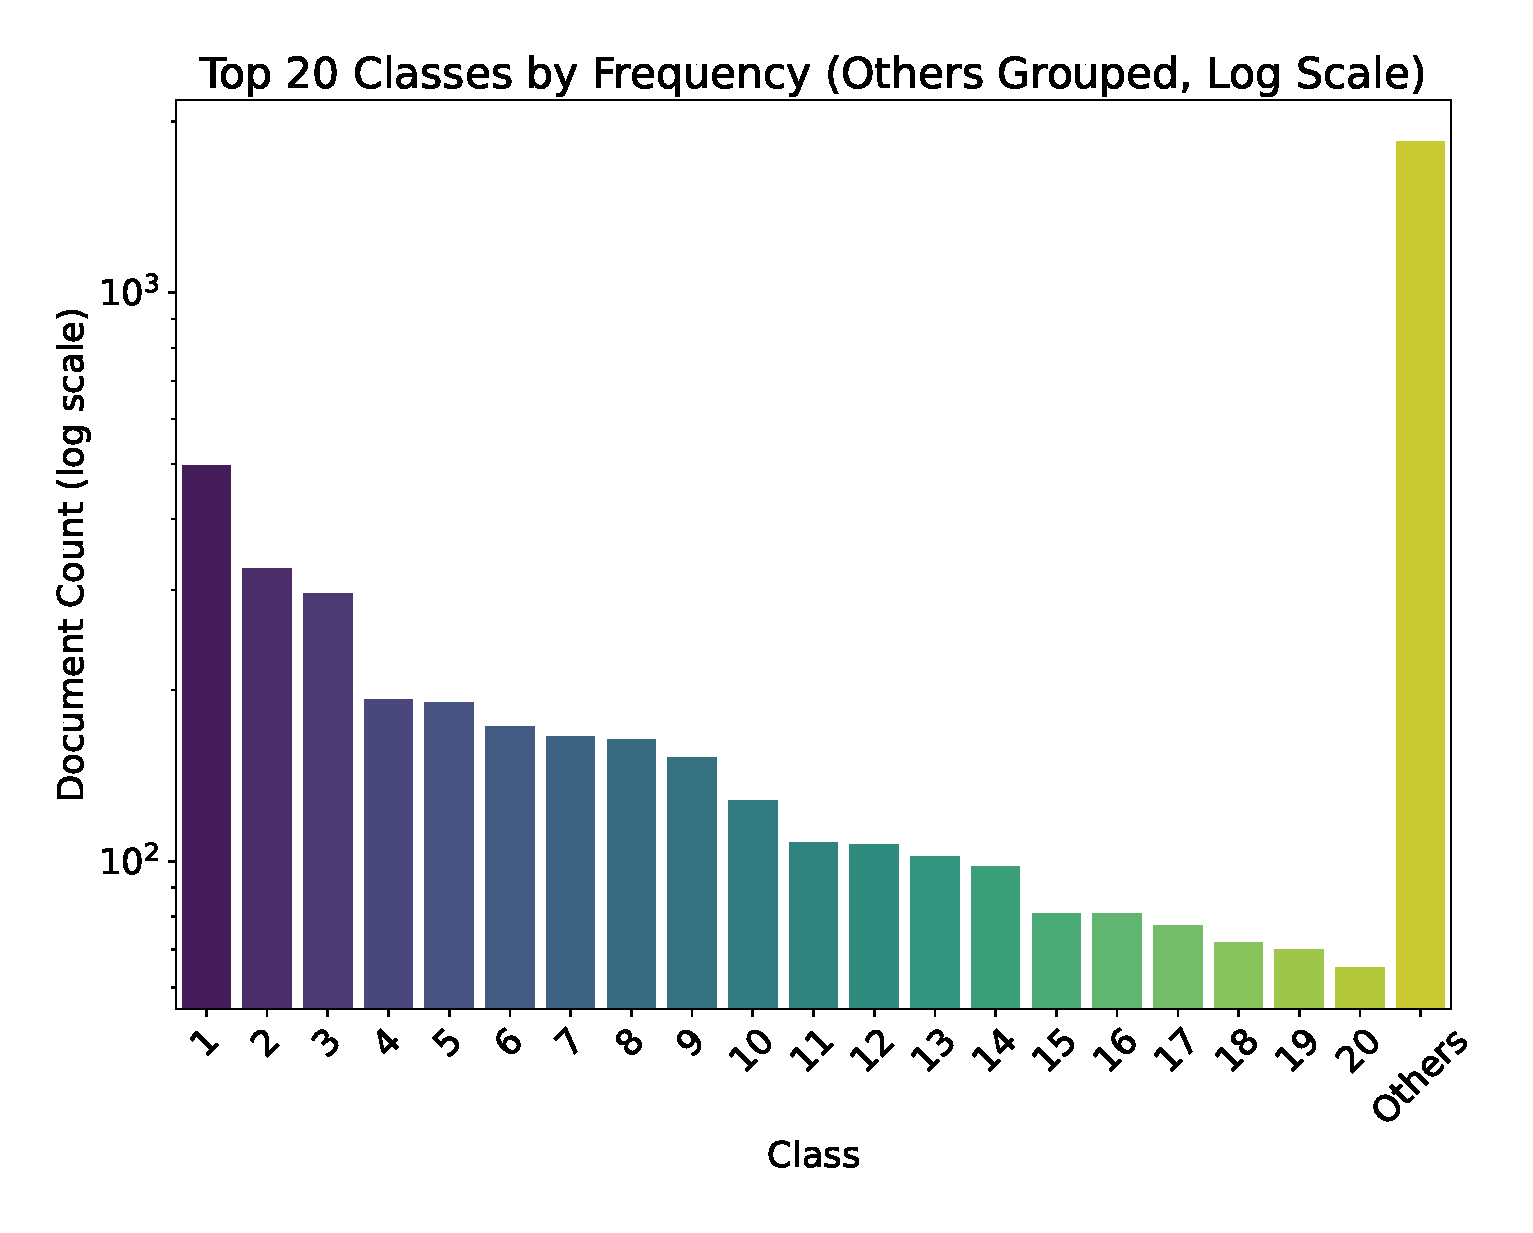
\includegraphics[width=.8\textwidth]{images/hist2.eps}
\caption{Histogram showing the top 20 classes by their frequency. The other 124 classes are grouped in the ``others'' column. Note that the plot is in log scale.}
\label{fig:histplot}
\end{figure}  

To maintain train-test data consistency, the data is split following the \gls{ZSL} and \gls{GZSL} protocols proposed by Xian et al. \cite{xian_zero-shot_2019} (see \refCap{sec:zsl}). In both scenarios, the data is split into train and test data, and the train data is further divided by a 5-fold cross-validation \cite{wong_reliable_2019}. The data for the test scenario and the data for each split are chosen randomly, and remain the same for every experiment. The test scenario is picked as a sixth split for the cross-validation, so it follows the same rules as the other five splits. For the \gls{ZSL} scenario, one-sixth of the classes are randomly chosen for each split, with no overlapping. Naturally, this scenario creates splits with variable sizes, as the classes themselves have variable sizes. For the \gls{GZSL} scenario, half the classes in the whole dataset are chosen as classes that do not overlap between splits, and the other half are distributed across the splits. While constructing a split, first the nonoverlapping classes are chosen for the split, then the remaining slots are filled with the overlapping classes, achieving splits with a constant size for this scenario.

This dataset can be normally used for a traditional visual classification problem, but since the problem is tackled with metric learning, additional considerations must be taken into account. While using a Siamese network, running inference on a single point of data returns no information, as the architecture requires some sort of comparison between different data points. Randomly selecting pairs every test can fluctuate the results, therefore, to maintain test consistency, a test protocol is used that ensures the same pairs are tested every time. For every document in the set, two other documents are chosen: one that shares the same class, and one that does not. This document is chosen randomly by its class, therefore, every class has the same probability of being picked. A protocol exists for the test set and for every cross-validation split.


\section{Evaluation Criteria}
\label{sec:evaluation}

Since a metric learning model yields a distance between two data points (in this case, two documents), a threshold needs to be defined to declare whether the two data points belong to the same class or not, to calculate how accurate the model is. For this, \gls{EER} is used as the metric for the experiments~\cite{agrawal_hybrid_2014}. \gls{EER} is the point at which the \gls{FAR} and \gls{FRR} are equal. The \gls{EER} is calculated by setting the \gls{FAR} equal to the \gls{FRR} and finding the corresponding threshold at this point~\cite{hofbauer_calculating_2016}. In other words, the \gls{EER} is the value of error rate when the threshold value $\tau_{EER}$ gives 
\begin{equation}
    FAR(\tau_{EER}) = FRR(\tau_{EER}),
\end{equation}
where
\begin{equation} \label{far}
    FAR(\tau) = \frac{\text{Number of false acceptances at threshold~} \tau}{\text{Total number of negative samples}}
\end{equation}
is the probability that a negative sample is incorrectly classified as positive. On the other hand,
\begin{equation} \label{frr}
    FRR(\tau) = \frac{\text{Number of false rejections at threshold~} \tau}{\text{Total number of positive samples}}
\end{equation}
is the probability that a positive sample (e.g., a genuine user) is incorrectly classified as negative.

Ten models are trained for each chosen backbone (see \refCap{sec:method_modeling}): a 5-fold cross-validation for each of the 2 scenarios, \gls{ZSL} and \gls{GZSL}. As shown in Section \ref{sec:method_dataset}, each split follows a fixed validation protocol to ensure consistency. The trained models from each split are also evaluated on the independent test set, to compare them with the \gls{LLM}s. The mean \gls{EER} is reported for every cross-validation scenario, as well as the mean \gls{EER} on the independent test set.

\section{VDM Experimental Setup}

The method was implemented in Python language, mainly using the PyTorch library~\cite{paszke_pytorch_2019}. The hyperparameters used in these experiments are shown on \refTab{tab:hyperparameters}. Note that, while most of the architectures use the same hyperparameter, MobileNetV3 and \gls{ViT} use different configurations, following suggestions from their original works.

\begin{table}[htbp]
\centering
\caption{Hyperparameters for different neural architectures in VDM experiments.}
\label{tab:hyperparameters}
\begin{tabular}{lccccc}
\hline
\textbf{Architecture} & \textbf{Optimizer} & \textbf{LR} & \textbf{LR Decay} & \textbf{WD} & \textbf{Epochs} \\
\hline
Default     & SGD   & 0.01  & Step (0.1/30 ep.)     & $1 \times 10^{-4}$ & 90 \\
MobileNetV3 & SGD   & 0.01  & Step (0.973/2 ep.)    & $1 \times 10^{-5}$ & 300 \\
ViT         & AdamW & 0.001 & Cosine Annealing      & $1 \times 10^{-5}$ & 90 \\
\hline
\end{tabular}
\end{table}

The VDM trained models are exclusively visual; therefore, their input data is the $(R, G, B)$ document image matrix. First, the input image is resized into a shape compatible with each neural architecture. For most models, this shape is $(224, 224)$ in height and width. EfficientNet is the only architecture that does not follow this rule, as the different model versions increase their input size at the same time they increase the network depth and width. Then, every value of the image matrix is scaled from $0\text{--}255$ to $0\text{--}1$, and normalized with the mean and standard deviation of the current training split.

\blue{During training, each step processes a pair of documents that can be either similar (same class) or dissimilar (different classes). The pairing process follows a specific procedure: first, a random document is selected from the training set; then, the pair type (similar or dissimilar) is randomly determined. For similar pairs, another document from the same class is chosen. For dissimilar pairs, a different class is randomly selected first, followed by a random document from that class. This class-level randomization ensures that every class has equal probability of forming dissimilar pairs, preventing overfitting to larger classes. To maintain balance during training, half of all pairs are similar and half are dissimilar. Each batch is composed of 16 pairs. Throughout an epoch, each document is chosen twice to compose the first position of the pair: once to make similar pairs, and another to make dissimilar pairs. While the loop training randomizes each pair each epoch, during test and validation, the pairs are fixed. The chosen pair is then processed by the siamese network, generating two feature vectors, which are evaluated by the contrastive loss function (see \refCap{sec:contrastive_loss}).}
